\documentclass[b4paper, landscape, dvipdfmx]{jsarticle}
%----- 必要なパッケージ -----
\usepackage{fancybox,ascmac,otf}
\usepackage{amssymb, amsthm}
\usepackage[leqno]{amsmath}
\usepackage{geometry}
\usepackage{multicol}
\usepackage{tcolorbox}
\usepackage{xcolor}
\usepackage{fancyhdr}
\usepackage{tikz}

% TikZライブラリ
\usetikzlibrary{
    positioning,
    arrows.meta,
    calc,
    shadows,
    shadows.blur,
    intersections,
    angles,
    quotes,
    decorations.pathmorphing
}

% tcolorboxライブラリ
\tcbuselibrary{skins, breakable, theorems}

\usepackage{enumitem}
\setlist[enumerate,1]{label=(\arabic*)}
\setlist[itemize]{leftmargin=*}
\newcommand{\ds}{\displaystyle}

%----- レイアウト設定 -----
\geometry{
  left=15mm,
  right=15mm,
  top=20mm,
  bottom=15mm,
  headheight=25pt
}

%----- 数式環境の上下の余白調整 -----
\AtBeginDocument{
  \setlength{\abovedisplayskip}{5pt}
  \setlength{\belowdisplayskip}{5pt}
  \setlength{\abovedisplayshortskip}{0pt}
  \setlength{\belowdisplayshortskip}{3pt}
}

%===========================================================
%  デザイン設定
%===========================================================

%--- 色の定義 ---
\definecolor{printBlue}{RGB}{0, 50, 100}     % 濃紺
\definecolor{printRed}{RGB}{140, 20, 20}     % 濃エンジ
\definecolor{printTeal}{RGB}{0, 60, 60}      % 濃い青緑

%--- 共通スタイル定義 ---
\tcbset{
    chartbox/.style={
        enhanced,
        fonttitle=\sffamily\bfseries,
        boxrule=1pt,
        arc=2pt,
        top=1.0em,
        nobeforeafter,
        enlarge left by=-2mm,
        enlarge right by=-2mm,
        drop fuzzy shadow,
        colback=white,
        attach boxed title to top left={xshift=10pt, yshift*=-\tcboxedtitleheight/2},
        boxed title style={frame hidden, sharp corners, rounded corners=southeast, arc=3pt}
    }
}

%--- 各種ボックス環境定義 ---
\newtcolorbox{any}[1]{
    enlarge left by=0mm, enlarge right by=0mm,
    enhanced, frame hidden, colback=white, title={#1},
    attach boxed title to top left={xshift=0mm, yshift=0mm},
    coltitle=white, fonttitle=\bfseries\sffamily,
    boxed title style={
        colback=black!80, frame hidden, arc=4pt, outer arc=4pt,
        sharp corners=south, boxrule=0pt,
        top=1mm, bottom=1mm, left=3mm, right=3mm
    },
    underlay boxed title={
        \draw[thick, black!80] (title.south west) -- (title.south west-|frame.east);
    },
    breakable, top=5mm, left=2mm, right=2mm, bottom=0mm,
    before skip=1em, after skip=1em,
    segmentation style={draw=black!40, dashed}
}

\newtcolorbox{eg}[1]{
    chartbox,
    colframe=printBlue,
    coltitle=white,
    title=\textbf{例題 #1},
    boxed title style={colback=printBlue},
    segmentation style={draw=printBlue, line width=0.5pt, dashed}
}

\newtcolorbox{prac}[1]{
    chartbox,
    colframe=printRed,
    coltitle=white,
    title=\textbf{練習 #1},
    boxed title style={colback=printRed}
}

\newtcolorbox{thm}[1]{
    chartbox,
    colframe=printTeal,
    coltitle=white,
    title=\textbf{#1},
    boxed title style={colback=printTeal}
}

\newtcolorbox{answer}[1][height fill]{
    enhanced,
    title={Memo / Answer},
    colframe=black!80,
    colback=white,
    coltitle=black!60,
    fonttitle=\sffamily\bfseries,
    attach boxed title to top left={xshift=5mm, yshift*=-\tcboxedtitleheight/2},
    boxed title style={frame hidden, colback=white},
    boxrule=1pt,
    arc=1pt,
    nobeforeafter,
    enlarge left by=-2mm, 
    enlarge right by=-2mm, 
    height fill,
    segmentation style={draw=black!20, solid},
    underlay={
        \begin{tcbclipinterior}
            \draw[step=5mm, black!5, ultra thin] (interior.south west) grid (interior.north east);
        \end{tcbclipinterior}
    }, 
    #1
}

%----- ヘッダーの設定 -----
\pagestyle{fancy}
\fancyhf{}
\fancyhead[C]{%
    \begin{tikzpicture}[remember picture, overlay]
        \node[anchor=north west, fill=printBlue, minimum width=\paperwidth, minimum height=5pt] at (current page.north west) {};
    \end{tikzpicture}
}
\fancyhead[L]{\small \textcolor{black!90}{数学C $>$ 第1章--平面ベクトル $>$ 第10回 \textbf{ベクトル方程式(直線)}}}
\fancyhead[R]{\small 年 \hspace{1cm} 組 \hspace{1cm} 番 \quad 氏名 \hspace{6cm}}
\renewcommand{\headrulewidth}{0pt}

\begin{document}

%=============================================================================
% 1枚目:ベクトル方程式の概念
%=============================================================================
\begin{multicols}{2}

%-----------------------------------------------------------------------------
% 左カラム:図形の方程式とは
%-----------------------------------------------------------------------------
\begin{any}{1. (復習)そもそも「図形の方程式」とは?}
    数学IIで習った「直線の方程式 $y=2x+1$」とは何だっただろうか.
    
    \begin{thm}{図形の定義}
        図形とは, \textbf{ある条件を満たす「点」全体の集合} である.
    \end{thm}
    \begin{minipage}{0.48\textwidth}
        例えば $y=2x+1$ は, 
    「$x$座標を2倍して1足すと$y$座標になる」という条件を満たす点 $(x, y)$ を無数に集めると, 一本の直線になることを意味している.
    \end{minipage}
    \begin{minipage}{0.5\textwidth}
    \vspace{0.5cm}
          \begin{center}
    \begin{tikzpicture}[scale=0.8]
        \draw[->, gray] (-1,0) -- (4,0) node[right]{$x$};
        \draw[->, gray] (0,-1) -- (0,4) node[above]{$y$};
        \draw[thick, printBlue] (-0.5, 0) -- (1.5, 4);
        \fill (0,1) circle (2pt);
        \fill (1,3) circle (2pt);
        \fill (0.5, 2) circle (2pt);
        \node[right] at (1.5, 4) {点の集まり};
    \end{tikzpicture}
    \end{center}
    \end{minipage}
\end{any}
\begin{any}{2. 点とベクトルの同一視}
    位置ベクトルを導入したことで, 我々は次の対応関係を手に入れた.
    \[ \text{点 P} \longleftrightarrow \text{位置ベクトル } \vec{p} \ (\text{原点Oからの矢印}) \]
    
    これにより, 「点 P が満たす条件」を「ベクトル $\vec{p}$ が満たす条件」に書き換えることができる. これが\textbf{ベクトル方程式}である.

    \begin{thm}{ベクトル方程式}
        変数ベクトル $\vec{p}$ が満たすべき等式のこと.
        この等式を満たす $\vec{p}$ の終点 P 全体が作る図形を考える.
    \end{thm}

    \textbf{イメージ:} 
    条件を満たすような矢印 $\vec{p}$ を無数に描いたとき, その「矢印の先端(終点)」が描く軌跡が図形となる.
    
    \begin{center}
    \begin{tikzpicture}[scale=1.0, >=stealth]
        \coordinate (O) at (0,0);
        % Line
        \draw[ultra thick, printBlue!20] (-1, 2.5) -- (4, 1.5);
        \node[printBlue, above] at (3.5, 1.6) {直線 $l$};
        
        % Sample vectors
        \draw[->, thick, printTeal] (O) -- (0, 2.3);
        \draw[->, thick, printTeal] (O) -- (1, 2.1);
        \draw[->, thick, printTeal] (O) -- (2, 1.9);
        \draw[->, thick, printTeal] (O) -- (3, 1.7) node[right] {$\vec{p}$};
        
        \fill (O) circle (2pt) node[below left] {O};
        \node[align=left, scale=0.9] at (2, -1) {
            条件を満たす矢印の\\
            \textbf{先端}が直線を形作る.
        };
    \end{tikzpicture}
    \end{center}
\end{any}

\columnbreak

\end{multicols}

%=============================================================================
% 2枚目:方向ベクトルによる直線
%=============================================================================
\newpage
\begin{multicols}{2}

%-----------------------------------------------------------------------------
% 左カラム:方向ベクトルの導入
%-----------------------------------------------------------------------------
\begin{any}{3. 「1点」と「向き」で決まる直線}
    最も基本的な直線の定義は, 「通る点A」と「進む方向 $\vec{d}$」を指定することである.
    
    点 P($\vec{p}$) がこの直線上にある条件は,
    \[ \overrightarrow{\text{AP}} // \vec{d} \quad (\text{平行}) \]
    である. つまり, ある実数 $t$ を用いて $\overrightarrow{\text{AP}} = t\vec{d}$ と書ける.
    
    これを用いて $\vec{p}$ を表すと:
    \[ \vec{p} = \overrightarrow{\text{OA}} + \overrightarrow{\text{AP}} = \vec{a} + t\vec{d} \]

    \begin{thm}{直線のベクトル方程式 (方向ベクトル)}
        定点 A($\vec{a}$) を通り, 方向ベクトル $\vec{d}$ に平行な直線:
        \[ \vec{p} = \vec{a} + t\vec{d} \quad (t \text{は実数}) \]
    \end{thm}
    
    \begin{center}
    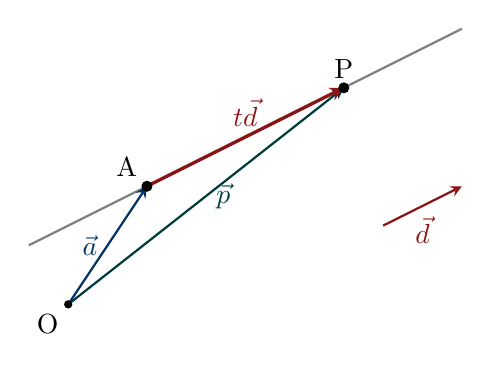
\begin{tikzpicture}[scale=1.0, >=stealth]
        \coordinate (O) at (0, -0.5);
        \coordinate (A) at (1, 1);
        \coordinate (P) at (3.5, 2.25); % t=2.5 approx
        
        % Line
        \draw[thick, gray] (-0.5, 0.25) -- (5, 3);
        
        % Vectors
        \draw[->, thick, printBlue] (O) -- (A) node[midway, left] {$\vec{a}$};
        \draw[->, thick, printTeal] (O) -- (P) node[midway, right] {$\vec{p}$};
        
        % Direction on line
        \draw[->, very thick, printRed] (A) -- (P) node[midway, above] {$t\vec{d}$};
        
        % Base direction vector d (shown separately)
        \draw[->, thick, printRed] (4, 0.5) -- (5, 1) node[midway, below] {$\vec{d}$};
        
        \fill (A) circle (2pt) node[above left] {A};
        \fill (P) circle (2pt) node[above] {P};
        \fill (O) circle (1.5pt) node[below left] {O};
    \end{tikzpicture}
    \end{center}

    直線APとは,ある実数$t$を用いて,
    \[\vec{p}=\vec{a}+t\vec{d}\]
    と書けるようなベクトル全体の集合のことである.
\end{any}

%-----------------------------------------------------------------------------
% 右カラム:媒介変数表示
%-----------------------------------------------------------------------------
\columnbreak

\begin{any}{4. 成分(座標)との関係}
    ベクトル方程式 $\vec{p} = \vec{a} + t\vec{d}$ を成分で書いてみる.
    \begin{itemize}
        \item 通る点: $\vec{a} = (x_1, y_1)$
        \item 方向ベクトル: $\vec{d} = (l, m)$
        \item 直線上の点: $\vec{p} = (x, y)$
    \end{itemize}
    代入すると:
    \[ (x, y) = (x_1, y_1) + t(l, m) = (x_1+lt, \ y_1+mt) \]
    
    \begin{thm}{直線の媒介変数表示}
        \[
        \begin{cases}
            x = x_1 + lt \\
            y = y_1 + mt
        \end{cases}
        \]
    \end{thm}
    ここから $t$ を消去すると, 見慣れた $y - y_1 = \frac{m}{l}(x - x_1)$ などの式が得られる.

    \begin{eg}{1 (2点を通る直線)}
        2点 $A(2, 3), B(4, 7)$ を通る直線の方程式を求めよ.
        \tcblower
        \textbf{方針:}
        方向ベクトル $\vec{d}$ は $\overrightarrow{\text{AB}}$ である.
        $\vec{d} = (4-2, 7-3) = (2, 4)$.
        $\vec{p} = \vec{a} + t\vec{d}$ に代入する.
        \vspace{6cm}
    \end{eg}
\end{any}

\end{multicols}

%=============================================================================
% 3枚目:法線ベクトルによる直線
%=============================================================================
\newpage
\begin{multicols}{2}

%-----------------------------------------------------------------------------
% 左カラム:法線ベクトルの導入
%-----------------------------------------------------------------------------
\begin{any}{5. 「1点」と「垂直な向き」で決める直線}
    もう一つの直線の決め方は, 「通る点A」と「直線の\textbf{傾きに垂直なベクトル} $\vec{n}$」を指定することである.
    この $\vec{n}$ を\textbf{法線(ほうせん)ベクトル}という.

    点 P($\vec{p}$) が直線上にある条件は,
    \[ \overrightarrow{\text{AP}} \perp \vec{n} \quad (\text{または } \overrightarrow{\text{AP}}=\vec{0}) \]
    である. これを内積を用いて表すと:
    \[ \vec{n} \cdot \overrightarrow{\text{AP}} = 0 \]
    
    \begin{thm}{直線のベクトル方程式 (法線ベクトル)}
        定点 A($\vec{a}$) を通り, 法線ベクトル $\vec{n}$ を持つ直線:
        \[ \vec{n} \cdot (\vec{p} - \vec{a}) = 0 \]
    \end{thm}
    
    \begin{center}
    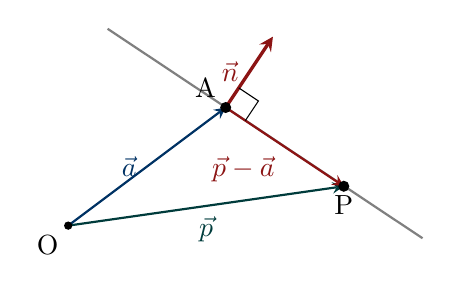
\begin{tikzpicture}[scale=1.0, >=stealth]
        \coordinate (O) at (0, -0.5);
        \coordinate (A) at (2, 1);
        \coordinate (P) at (3.5, 0); 
        \coordinate (N) at (2.6, 1.9); 
        
        % Line
        \draw[thick, gray] (0.5, 2) -- (4.5, -0.66);
        
        % Vectors
        \draw[->, thick, printBlue] (O) -- (A) node[midway, left] {$\vec{a}$};
        \draw[->, thick, printTeal] (O) -- (P) node[midway, below] {$\vec{p}$};
        \draw[->, thick, printRed] (A) -- (P) node[midway, below left] {$\vec{p}-\vec{a}$};
        
        % Normal vector
        \draw[->, very thick, printRed] (A) -- (N) node[midway, left] {$\vec{n}$};
        
        % Angle
        \pic [draw, angle radius=3mm] {right angle = P--A--N};

        \fill (A) circle (2pt) node[above left] {A};
        \fill (P) circle (2pt) node[below] {P};
        \fill (O) circle (1.5pt) node[below left] {O};
    \end{tikzpicture}
    \end{center}
\end{any}

%-----------------------------------------------------------------------------
% 右カラム:一般形との接続
%-----------------------------------------------------------------------------
\columnbreak

\begin{any}{6. 一般形 $ax+by+c=0$ の正体}
    法線ベクトルの式を成分で計算してみよう.
    $\vec{n}=(a, b), A(x_1, y_1), P(x, y)$ とする.
    
    \[ \vec{n} \cdot (\vec{p} - \vec{a}) = 0 \]
    \[ (a, b) \cdot (x-x_1, \ y-y_1) = 0 \]
    \[ a(x-x_1) + b(y-y_1) = 0 \]
    
    これを展開すると:
    \[ ax + by - ax_1 - by_1 = 0 \]
    $-ax_1 - by_1$ は定数なので $c$ と置くと, 直線の方程式 $ax+by+c=0$ になる!
    
    \begin{tcolorbox}[colback=yellow!10, frame hidden, title={係数の正体}]
        直線の方程式 $ax+by+c=0$ における $x, y$ の係数ベクトル $(a, b)$ は, 
        その直線の\textbf{法線ベクトル}を表している.
    \end{tcolorbox}

    \begin{eg}{2 (法線ベクトルの利用)}
        点 $A(3, 1)$ を通り, $\vec{n}=(2, -5)$ に垂直な直線の方程式を求めよ.
        \tcblower
        \textbf{解法:} 
        法線が $(2, -5)$ なので, 直線の式は $2x - 5y + c = 0$ の形になる.
        あとは点Aを通ることから決定する.
        (ベクトル方程式 $\vec{n}\cdot(\vec{p}-\vec{a})=0$ に直接代入してもよい)
        \vspace{8cm}
    \end{eg}
\end{any}

\end{multicols}

%=============================================================================
% 4枚目:確認テスト(問題)
%=============================================================================
\newpage
\fancyhead[L]{\small \textcolor{black!90}{数学C $>$ 第1章--平面ベクトル $>$ 第10回--\textbf{確認テスト}}}
\begin{multicols}{2}

\begin{any}{確認テスト (A: 基本)}
    \begin{prac}{A1 (方向ベクトル)}
        点 $A(-1, 2)$ を通り, ベクトル $\vec{d}=(3, -4)$ に平行な直線 $l$ を考える.
        \begin{enumerate}
            \item 直線 $l$ 上の点 $(x, y)$ を, 媒介変数 $t$ を用いて表せ.
            \item $t$ を消去して $x, y$ の方程式を求めよ.
        \end{enumerate}
    \end{prac}
    \begin{answer}[height=6cm]
    \end{answer}

    \begin{prac}{A2 (法線ベクトル)}
        次の直線の方程式を求めよ.
        \begin{enumerate}
            \item 点 $(2, 3)$ を通り, ベクトル $\vec{n}=(4, -1)$ に垂直な直線.
            \item 直線 $2x + 3y - 5 = 0$ に垂直なベクトル(法線ベクトル)を1つ答えよ.
        \end{enumerate}
    \end{prac}
    \begin{answer}[height=6cm]
    \end{answer}
\end{any}

\columnbreak

\begin{any}{確認テスト (B: 標準)}
    \begin{prac}{B1 (2点を通る直線と法線)}
        2点 $A(1, 4), B(5, 2)$ を通る直線 $l$ について以下の問いに答えよ.
        \begin{enumerate}
            \item 直線 $l$ の方向ベクトル $\vec{d}$ を求めよ.
            \item 直線 $l$ の法線ベクトル $\vec{n}$ を1つ求めよ. (成分は整数でよい)
            \item 点 $P(2, 1)$ から直線 $l$ に下ろした垂線の足を $H$ とする. $H$ の座標を求めよ.
        \end{enumerate}
    \end{prac}
    \begin{answer}[height=10cm]
    \end{answer}
\end{any}

\end{multicols}

%=============================================================================
% 5枚目:確認テスト(解答)
%=============================================================================
\newpage
\fancyhead[L]{\small \textcolor{black!90}{数学C $>$ 第1章--平面ベクトル $>$ 第10回 \textbf{【解答解説】}}}

\begin{multicols}{2}

\begin{any}{解答 (A: 基本)}
    \begin{prac}{A1 解答}
        (1) $\vec{p} = \vec{a} + t\vec{d}$ より,
        \[ (x, y) = (-1, 2) + t(3, -4) \]
        よって, $\boldsymbol{\begin{cases} x = -1 + 3t \\ y = 2 - 4t \end{cases}}$
        
        (2) $t$ を消去する.
        第1式より $3t = x+1 \implies t = \frac{x+1}{3}$.
        第2式へ代入: $y = 2 - 4(\frac{x+1}{3})$.
        $3y = 6 - 4(x+1) \implies 3y = 6 - 4x - 4$.
        $\boldsymbol{4x + 3y - 2 = 0}$
        
        \textbf{別解:} 方向ベクトル $(3, -4)$ より傾きは $-\frac{4}{3}$.
        $y - 2 = -\frac{4}{3}(x - (-1))$ を整理してもよい.
    \end{prac}

    \begin{prac}{A2 解答}
        (1) 法線ベクトルが $\vec{n}=(4, -1)$ なので, 求める直線の式は
        $4(x - 2) - 1(y - 3) = 0$
        $4x - 8 - y + 3 = 0$
        $\boldsymbol{4x - y - 5 = 0}$
        
        (2) 直線 $ax+by+c=0$ の法線ベクトルは $(a, b)$ である.
        よって $\boldsymbol{\vec{n} = (2, 3)}$ (またはその実数倍)
    \end{prac}
\end{any}

\columnbreak

\begin{any}{解答 (B: 標準)}
    \begin{prac}{B1 解答}
        (1) 方向ベクトルは $\overrightarrow{\text{AB}}$.
        \[ \vec{d} = (5-1, 2-4) = (4, -2) \]
        簡単にするため $2$ で割って $\boldsymbol{\vec{d}=(2, -1)}$ としてもよい.
        
        (2) $\vec{d}=(2, -1)$ に垂直なベクトル $\vec{n}=(a, b)$ を探す.
        内積が0になればよい: $2a - b = 0$.
        例えば $a=1, b=2$ とすれば成り立つ.
        よって $\boldsymbol{\vec{n} = (1, 2)}$ (例).
        
        (3) 垂線の足 $H$ の求め方.
        $H$ は直線 $l$ 上にあるので, 方向ベクトル $\vec{d}=(2, -1)$ を用いて
        $H(1+2k, \ 4-k)$ (点Aを通り $\vec{d}$ 方向)とおける.
        
        $\overrightarrow{\text{PH}} \perp \vec{d}$ である.
        $\overrightarrow{\text{PH}} = \overrightarrow{\text{OH}} - \overrightarrow{\text{OP}} = (1+2k-2, \ 4-k-1) = (2k-1, \ 3-k)$.
        
        垂直条件より内積が0:
        \[ \overrightarrow{\text{PH}} \cdot \vec{d} = 0 \]
        \[ (2k-1) \cdot 2 + (3-k) \cdot (-1) = 0 \]
        \[ 4k - 2 - 3 + k = 0 \implies 5k = 5 \implies k = 1 \]
        
        $k=1$ を $H$ の座標に代入して,
        $H(1+2(1), \ 4-1) = \boldsymbol{(3, 3)}$.
    \end{prac}
    
    \begin{tcolorbox}[colback=white, title={別解(法線ベクトルの利用)}]
        直線 $l$ の式は, $\vec{n}=(1, 2)$ と点A$(1, 4)$ より
        $1(x-1) + 2(y-4) = 0 \implies x+2y-9=0$.
        点 $P(2, 1)$ を通り, 直線 $l$ に垂直な直線 $m$ を求める.
        $m$ の方向ベクトルは $\vec{n}=(1, 2)$.
        $m: (x, y) = (2, 1) + s(1, 2) = (2+s, 1+2s)$.
        これを $l$ の式に代入して交点 $H$ を求める.
        $(2+s) + 2(1+2s) - 9 = 0 \implies 5s - 5 = 0 \implies s=1$.
        よって $H(3, 3)$.
    \end{tcolorbox}
\end{any}

\end{multicols}
\end{document}